\documentclass[../../Rapport RayTracer.tex]{subfiles}


\begin{document}


Afin de rendre les réflexions de la scène plus remarquables et cette dernière moins monotone, nous avons implémenté un damier au sol au moyen d'UV mapping. Ainsi, pour chaque point d'intersection avec le plan représentant le sol, nous regardons si la somme des coordonnées X et Y du point d'intersection est paire ou non. Si la somme est paire, nous renverrons la première couleur du damier. Si elle est impaire, nous renverrons alors la deuxième couleur du damier.\\

\begin{figure}[h!]
	\adjustbox{center}
	{
		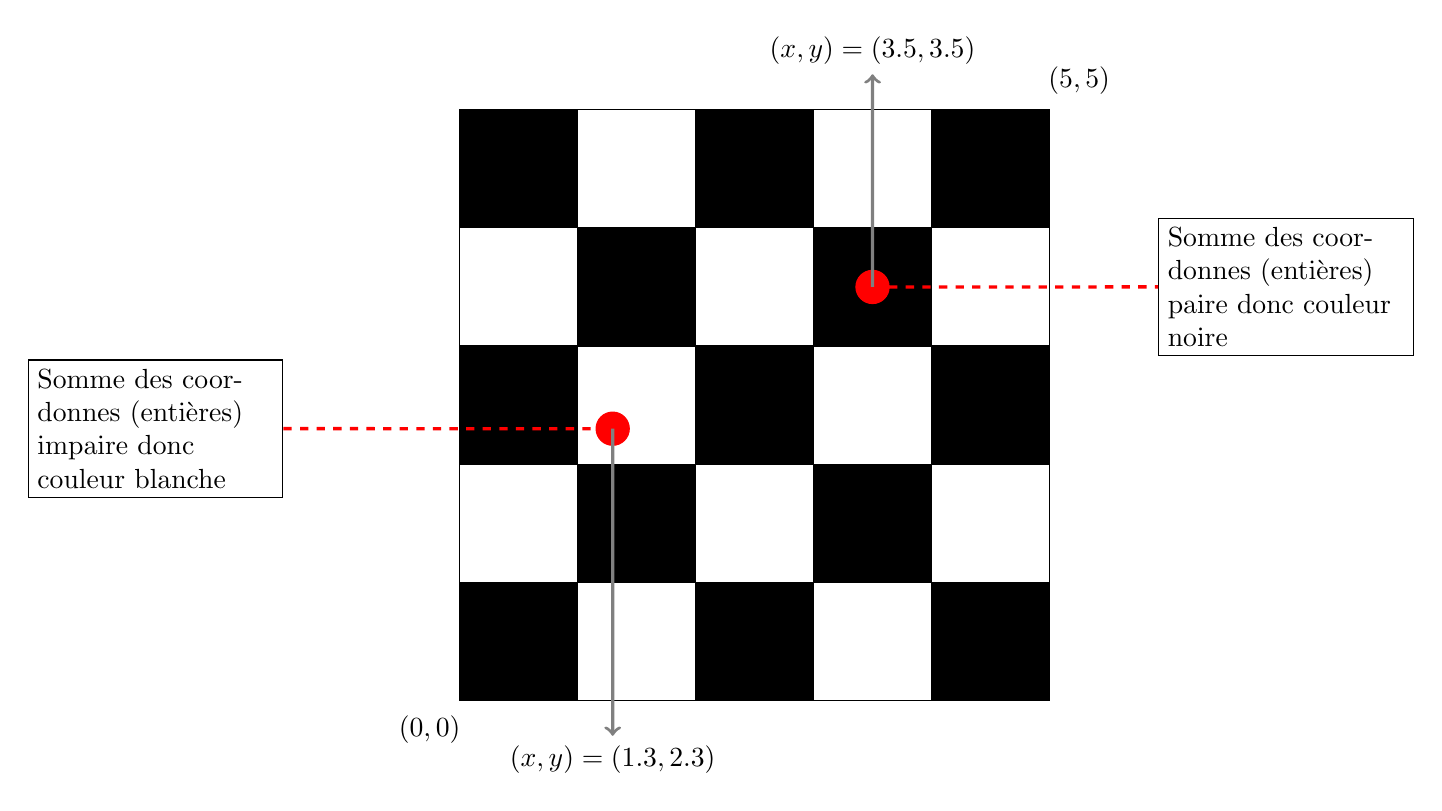
\begin{tikzpicture}[scale=1.5]
			%Dessin du damier
			\foreach \row in {0, 1, 2, ..., 4} 
			{
				\foreach \column in {0, 1, 2, ..., 4}
				{
					\pgfmathparse{Mod(\row + \column, 2) ? "white" : "black"}%On calcule le résultat de ligne + colonne modulo 2
					\colorlet{couleurDamier}{\pgfmathresult}%On transforme la chaîne de caractère donnée par pgfmathparse en couleur

					\fill[color=couleurDamier] (\row, \column) rectangle (\row+1, \column+1);%On colorie la case de la grille tikz
				}
			} 

			%Grille pour afficher les bordures
			\draw (0, 0) grid (5, 5);

			%Point de coordonnées
			%Dimensions de la grille
			\node (coin 0 0) at (-0.25, -0.25) {$(0, 0)$};
			\node (coin 5 5) at (5.25, 5.25) {$(5, 5)$};

			%Points exemple
			\filldraw[color=red] (1.3, 2.3) circle (4pt);
			\filldraw[color=red] (3.5, 3.5) circle (4pt);

			%Explications
			\node[draw, text width=3cm] (exp 1) at (-2-2.5cm, 2.3) {Somme des coordonnes (entières) impaire donc couleur blanche};
			\node[draw, text width=3cm] (exp 2) at (7, 3.5) {Somme des coordonnes (entières) paire donc couleur noire};

			\node (coords 1) at (1.3, -0.5) {$(x, y) = (1.3, 2.3)$};
			\node (coords 2) at (3.5, 5.5) {$(x, y) = (3.5, 3.5)$};

			%Lignes
			\draw[dashed, color=red, very thick] (exp 1)--(1.3, 2.3);
			\draw[dashed, color=red, very thick] (3.5, 3.5)--(exp 2);

			\draw[->, color=black!50!white, very thick] (1.3, 2.3)--(coords 1);
			\draw[->, color=black!50!white, very thick] (3.5, 3.5)--(coords 2);
		\end{tikzpicture}
	}
\end{figure}
\FloatBarrier

Bien que simple, cet algorithme d'UV mapping nous a permis d'embrayer sur l'implémentation d'une skybox. Notre skybox n'est autre qu'une image équirectangulaire haute résolution d'un espace à ciel ouvert. Pour l'afficher correctement comme le ciel de notre scène, nous allons, là encore, utiliser un mécanisme d'UV mapping. C'est en effet un moyen simple de convertir les coordonnées d'un point sur une sphère hypothétique de rayon 1 (notre ciel) en des coordoonées 2D pour une image (notre image haute résolution).


\end{document}